\section{Introduction} \label{sec:introduction}

% What are containers and why they are becoming popular: pointing out portability and resource efficiency.

Containerization is a critical trend of applications running in data centers.
By wrapping a process into a complete filesystem and namespace cell, a container
has everything needed to run the process, including executables, libraries, system
tools, configurations, etc., without relying on external dependencies.
 \vyas{not sure why this is unique to container .. VM offers the same thing to?}
 \harry{VM encapsulate an entire guest OS, while a container encapsulates a process and runs directly on host OS. Do we need to clarify here?} 
Therefore, one container
is highly portable to run on any host with a proper OS kernel, and independent
with other containers on the same host without naming or version conflicts.
Such {\em portability} and {\em independence} significantly simplifies 
the life cycle of a containerized application, from testing to high availability 
maintenance.

A containerized application usually have multiple containers which are 
deployed in a multi-host cluster and connected by networks. When a container
is inter-connected with other containers, its portability and independence 
also rely on the flexibility of the network. For instance, one method of 
container networking, called 
{\em Host} mode, is to bind each container to its host's IP
and port and let the containers to communicate via TCP/IP like ordinary 
processes.
However, Host mode networking breaks the independence of a container because
the container can have port conflicts with others in the same host, and also undermines
the portability of a container because the container's IP and port will be changed when
it is moved to another host. A container should be reachable with 
an IP address independent with its location and 
have the freedom to bind any ports. 
Currently, this requirement is achieved by {\em Overlay} networking mode
(see details in \S\ref{sec:motivation}).
%by making it
%coordinate with other containers in the same host to avoid port conflicts
%and undermines the portability of a container by forcing its peers to
%update the IP address and ports when it is moved to another host.
%Instead of Host mode, people prefer {\em Overlay} mode in container networking.
%In this mode, containers are connected via an overlay network which 
%is built by software network bridge and routers. Containers then use
%overlay IP to communicate, and each container can keep its overlay IP
%no matter which host it is located.  
\vyas{getting a bit too low level for an intro. try to elevate 
it a bit and say this is status quo on the networking aspect}\harry{Simplified it.}

However, despite of the flexibility, we find in measurements that overlay
networks can easily become the performance bottleneck of containerized
applications. 
Figure~\ref{fig:intro-exist}(a) shows the network latency between two containers
on a single bare-metal host compared with two ordinary processes. 
We can see that overlay network has about 1.2 ms latency which is XXX orders
of magnitudes compared with ordinary processes and containers in Host mode.
Moreover, Figure~\ref{fig:intro-exist}(b) shows that overlay network can only
achieve about 20Gbps bandwidth between two containers on the same host 
which is about XX\% compared with ordinary processes and containers in Host mode.
In the bandwidth benchmarks, we also find that CPU is the bottleneck which 
limits the network throughput. As shown in Figure~\ref{fig:intro-exist}(b),
CPU are nearly saturated for processing the packets. Overall, the poor
performance and high overhead of overlay networks comes from the packet processing
burden to host OS kernel, and we will explain the performance penalty in more details in \S\ref{sec:motivation},
\vyas{not a fan of putting result graphs in intro. but if you feel this sells better .. we can keep it} \harry{You said you want to show measured evidence.
What do we put if we do not put graphs?}

\begin{figure}[t!]
     \centering 
     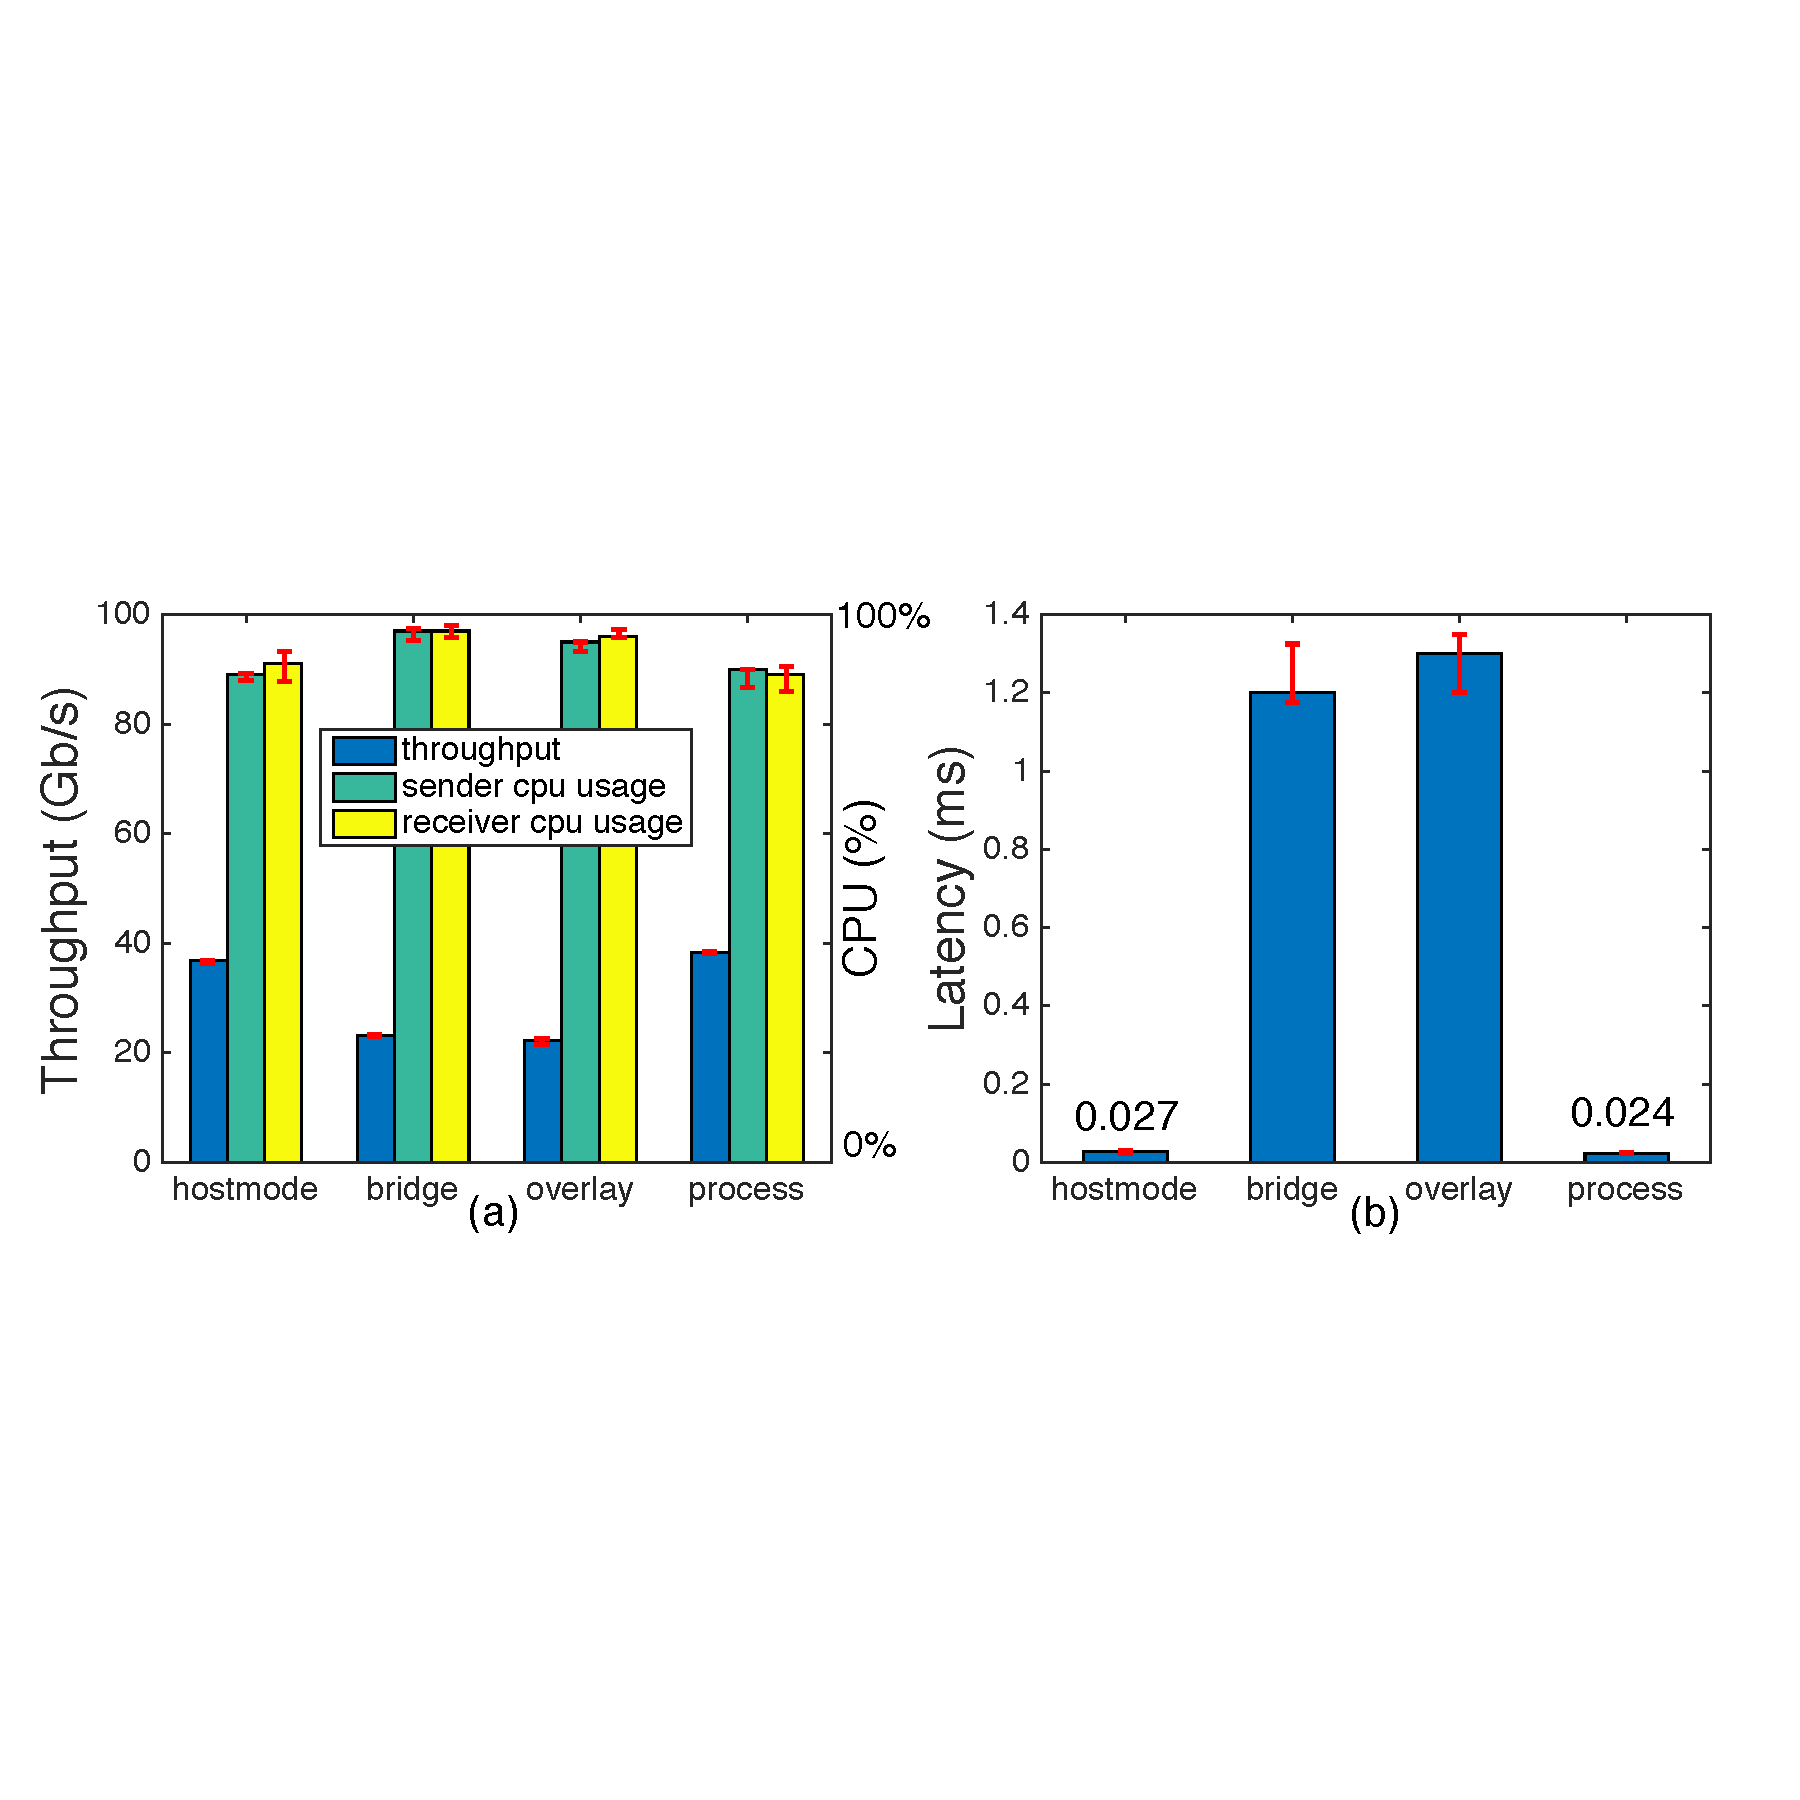
\includegraphics[width=0.46\textwidth]{figures/intro/intro_exist2.pdf} 
     \caption{Network latency, bandwidth and CPU overhead between containers compared with ordinary processes in a single bare-metal host. \harry{swap (a) and (b). remove bridge, because we can merge bridge and overlay.}}
     \label{fig:intro-exist}
\end{figure} 

The inefficiency of current container networking (overlay mode) 
will harm to applications which have high expectation  on network performance (e.g. < 5$\mu$s latency, > 40Gbps bandwidth~\cite{?}) in multiple aspects. 
On one hand,
it will significantly impact the overall performance of large scale distributed systems, such as big data analytics, key-value store, machine learning, and so on. On the other hand, it forces the applications to reserve substantial CPU
resources to merely perform traffic processing, which significantly raise the 
cost. Alternatively, people have to give up the portability and independence
of containers and go with the host mode. 

While the poor performance of an overlay (or virtual) network has been 
known and studied in VM networking~\cite{?}, containers make it uniquely challenging and perhaps impossible to adopt the existing solutions designed
for VM networking directly.
In the VM networking, one main stream solution to eliminate the inefficiency of the virtual networks is leveraging SR-IOV to let VMs directly talk to the NICs of hosts, bypassing the host OS kernel and hypervisor. 
However, SR-IOV cannot be directly applied on containers because containers 
do not have a hypervisor for SR-IOV to work with. In addition, one host can have
hundreds of containers which far exceeds the number of visualized NICs (\harry{how many?}) SR-IOV can support from a physical NIC. Furthermore, it is also not
favorable for containers to directly use kernel bypassing networking mechanisms like RDMA or DPDK, because the containers then will have to use te host mode.
\vyas{i dont understand what point this para is trying to make. lead in with the point you want to make -- e.g., While poor network i/o is not 
a new problem, containers make it uniquely challenging and perhaps impossible to adopt these directly .. Speciically..XYZ} \harry{Yeah, this is my point. Forgot to put the leading sentence. Fixed it.}

An ideal solution for container networking is an overlay network with flexible
IP assignment and routing in control-plane and high 
throughput, low latency and negligible overhead in data-plane. In this paper, we 
will discuss the opportunities and challenges to build such a solution. 
Specifically, with measurements, we first identify that the communications 
can be much more efficient if containers can transfer data via channels like
RDMA, DPDK \harry{maybe no time to do}, and shared-memory. However, to fully
realize the solution, we need to address several challenges. First of all, 
containers should use a standard API and overlay IP to communicate. The network
solution should be entirely transparent to them. Second, the overlay network
should avoid unnecessary memory copies when mapping the data transfer from
overlay network to physical network for efficiency; Finally, special optimizations, such as using shared-memory for intra-host networking, should be
implemented to push the performance to the limit. \vyas{this solution para doesnt sound like hotnets either.} \harry{So, how should it sound?}
